\title{バージョン管理システムチュートリアル}

\begin{document}

\begin{frame}
  \titlepage
\end{frame}

\section*{Outline}
\begin{frame}
  \tableofcontents
\end{frame}

\section{チュートリアルの概要}

\begin{frame}{VCSチュートリアル スタッフ}
  \begin{itemize}
  \item 講師
    \begin{itemize}
    \item 藤堂眞治 (東大物性研) \ \href{mailto:wistaria@issp.u-tokyo.ac.jp}{wistaria@issp.u-tokyo.ac.jp}
    \item 五十嵐 亮 (東大物性研) \ \href{mailto:rigarash@issp.u-tokyo.ac.jp}{rigarash@issp.u-tokyo.ac.jp}
    \item 松尾春彦 (RIST) \ \href{mailto:halm@rist.or.jp}{halm@rist.or.jp}
    \item 本山裕一 (東大院工) \ \href{mailto:yomichi@looper.t.u-tokyo.ac.jp}{yomichi@looper.t.u-tokyo.ac.jp}
    \end{itemize}
  \item 主催
    \begin{itemize}
    \item CMSI: 計算物質科学イニシアティブ \url{http://cms-initiative.jp/}
    \end{itemize}
  \item 共催
    \begin{itemize}
    \item RIST: 一般財団法人 高度情報科学技術研究機構 \url{http://www.rist.or.jp/}
    \end{itemize}
  \end{itemize}
\end{frame}

\begin{frame}
  \frametitle{チュートリアルの流れ}
  \begin{itemize}
    %\setlength{\itemsep}{1em}
  \item 準備作業
  \item バージョン管理システムとは? (講義 \& 実習)
  \item gitの基礎 (講義 \& 実習)
  \item ブランチとマージ (講義 \& 実習)
  \item リモートリポジトリとの連携 (講義 \& 実習)
  \item githubを用いたオープンソース・ソフトウェアの開発・公開 (講義 \& 実習)
  \item (optional) MateriAppsとMateriApps Live (講義)
  \item (optional) Gitをボトムアップから理解する (講義)
  \end{itemize}
\end{frame}

\section{準備作業}

\begin{frame}
  \frametitle{ネットワーク設定}
  \begin{itemize}
    %\setlength{\itemsep}{1em}
  \item LAN接続 (無線 or 有線)
  \item 実習用ワークステーションのアカウント登録
  \item github アカウント登録 (まだアカウントを持っていない人のみ)
    \begin{itemize}
    \item \url{https://github.com} にアクセス
    \item ``Sign up for GitHub''をクリック、必要事項を記入した後、``Create an account''
    \item SSH公開鍵の登録 (``Account settings'' $\Rightarrow$ ``SSH Keys'')
    \end{itemize} 
  \item sourceforge アカウント登録 (まだアカウントを持っていない人のみ)
    \begin{itemize}
    \item \url{http://sourceforge.net/} にアクセス
    \item 右上の``Join''をクリック、必要事項を記入して``Register''
    \end{itemize} 
  \end{itemize}
\end{frame}

\begin{frame}
  \frametitle{PCへのgitクライアントのインストール}
  \begin{itemize}
    \setlength{\itemsep}{1em}
  \item Windows \& Mac OX S
    \begin{itemize}
      \item \url{http://git-scm.com/downloads}からインストーラーをダウンロード
    \end{itemize}
  \item Linux \\
    \begin{minipage}{.9\textwidth}
      \begin{example}
        \$ sudo yum install git     \ \ \ \# Redhat系 \\
        \$ sudo apt-get install git \ \ \ \# Debian系
      \end{example}
    \end{minipage}
  \end{itemize}
\end{frame}

\section{バージョン管理システムの概要}

\begin{frame}
  \frametitle{diff と patch によるバージョン管理}
  \begin{itemize}
    \setlength{\itemsep}{1em}
  \item diff: 2つのテキストファイルの差分を出力するコマンド
    \begin{itemize}
    \item ファイル全体を保存するよりコンパクト
    \item 変更点を確認しやすい
    \end{itemize}
  \item patch: diff コマンドが生成した差分をファイルに適用するユーティリティー
    \begin{itemize}
    \item もとのファイルと差分から変更後のファイルを生成できる
    \end{itemize}
  \end{itemize}
\end{frame}

\begin{frame}
  \frametitle{実習: diff \& patch (1)}
  \begin{itemize}
    %\setlength{\itemsep}{1em}
  \item 単一ファイルの例
    \begin{minipage}{.9\textwidth}
      \begin{example}
        \$ cp /home/hands-on/vcs/diff/test.txt test.txt \\
        \$ cp test.txt test-orig.txt \\
        test.txt を編集 \\
        \$ diff -u test-orig.txt test.txt $>$ test.diff \\
        test.diff の中身を見てみる \\
        \$ mv test-orig.txt test.txt \\
        \$ patch $<$ test.diff \\
        test.txt の中身を確認
      \end{example}
    \end{minipage}
  \end{itemize}
\end{frame}

\begin{frame}
  \frametitle{実習: diff \& patch (2)}
  \begin{itemize}
    %\setlength{\itemsep}{1em}
  \item ディレクトリ全体を扱う例
    \begin{minipage}{.9\textwidth}
      \begin{example}
        \$ cp -rp /home/hands-on/vcs/diff testdir \\
        \$ cp -rp testdir testdir.orig \\
        testdir の中のファイルを編集 (ファイルの削除、追加も可) \\
        \$ diff -urN testdir.orig testdir $>$ testdir.diff \\
        testdir.diff の中身を見てみる \\
        \$ rm -rf testdir \&\& mv testdir.orig testdir \\
        \$ patch -p0 $<$ testdir.diff \\
        testdir の中身を確認
      \end{example}
    \end{minipage}
  \end{itemize}
\end{frame}

\begin{frame}
  \frametitle{バージョン管理システムとは?}
  \begin{columns}[T]
    \begin{column}{.7\textwidth}
      \begin{itemize}
        \setlength{\itemsep}{1em}
      \item ファイルの履歴をデータベース(リポジトリ)で一括管理するシス
        テム
      \item もともとはプログラムのソースコードのためのシステム
        \begin{itemize}
        \item それ以外のファイル(例えば \LaTeX ファイル)管理にも使える
        \end{itemize}
      \item 一人で使っても複数人で使っても超便利
        \begin{itemize}
        \item 超優秀な秘書のようなもの
        \end{itemize}
      \end{itemize}
    \end{column}
    \begin{column}{.25\textwidth}
      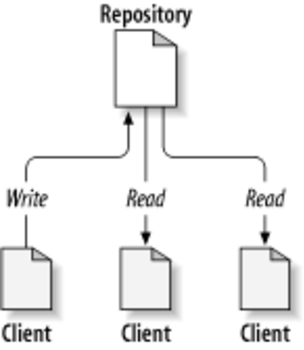
\includegraphics[width=\textwidth]{ch02dia1.pdf}
    \end{column}
  \end{columns}
\end{frame}

\begin{frame}
  \frametitle{なぜバージョン管理システムが必要なのか?}
  \begin{columns}[T]
    \begin{column}{.7\textwidth}
      \begin{itemize}
        \setlength{\itemsep}{1em}
      \item 作業者 and/or 作業場所が複数になると、ファイル名や手書きのログファイルによるバージョン管理はすぐに破綻する
        \begin{itemize}
        \item ネットワーク経由でファイルを check out/check in
        \item 更新毎に一意なバージョン番号 (リビジョン) を付与
        \item 任意のバージョン間の比較が容易
        \item バックアップの代わりにも
        \end{itemize}
      \item 複数箇所から同時に更新した場合に衝突を回避するしくみを備えている
      \item ブランチ・マージ・タグ付けなどが可能
      \end{itemize}
    \end{column}
    \begin{column}{.25\textwidth}
      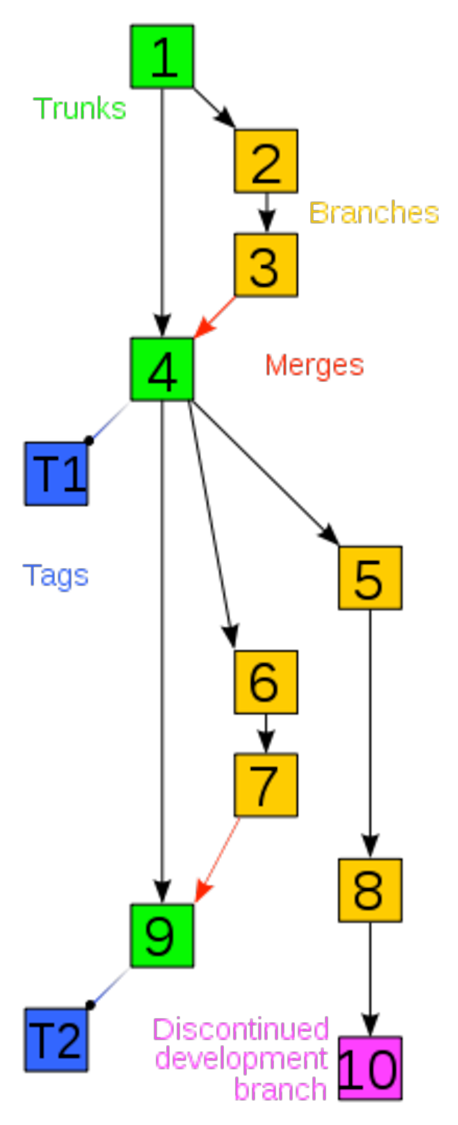
\includegraphics[width=.7\textwidth]{220px-Revision_controlled_project_visualization-2010-24-02.pdf}
    \end{column}
  \end{columns}
\end{frame}

\begin{frame}
  \frametitle{ありがちなパターン}
  \begin{center}
    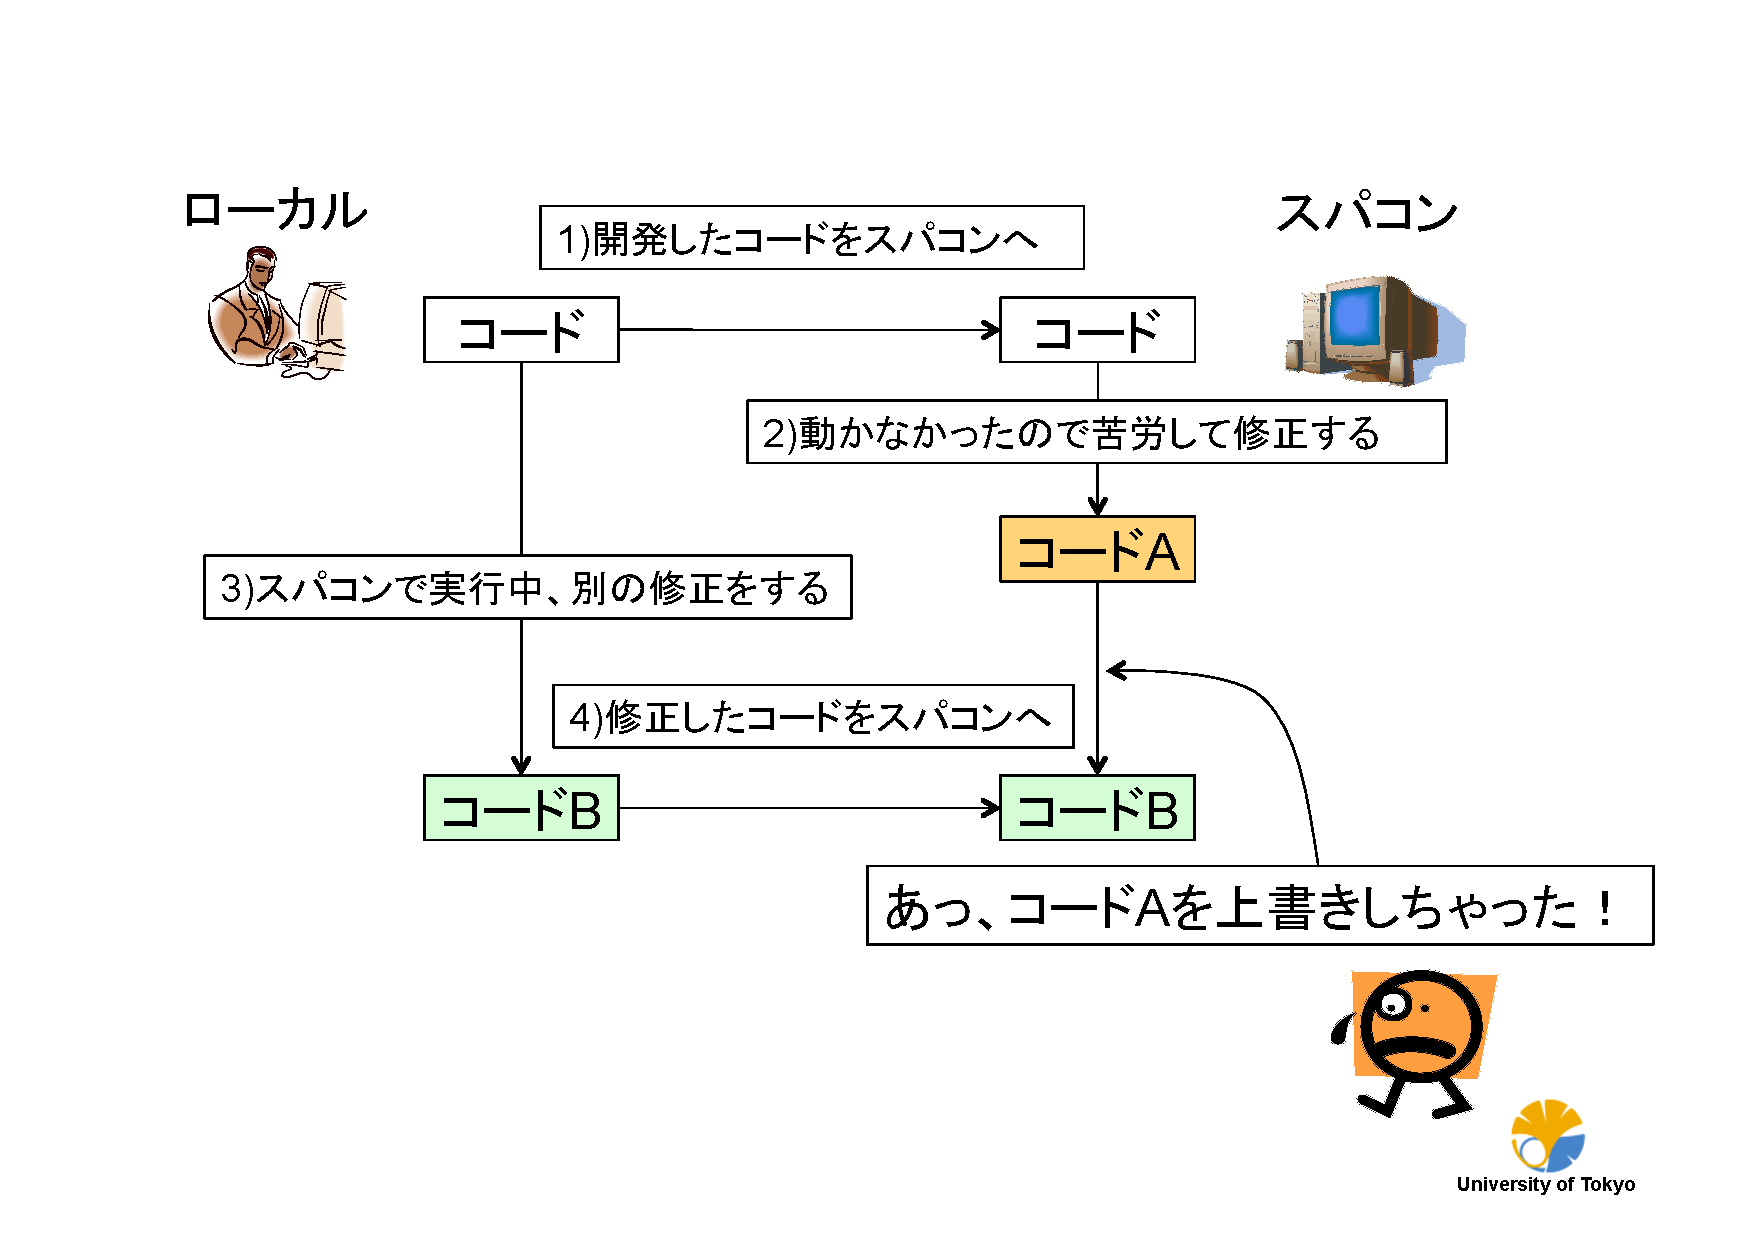
\includegraphics[height=0.88\textheight]{pattern-1.pdf}
  \end{center}
\end{frame}

\begin{frame}
  \frametitle{バージョン管理している場合}
  \begin{center}
    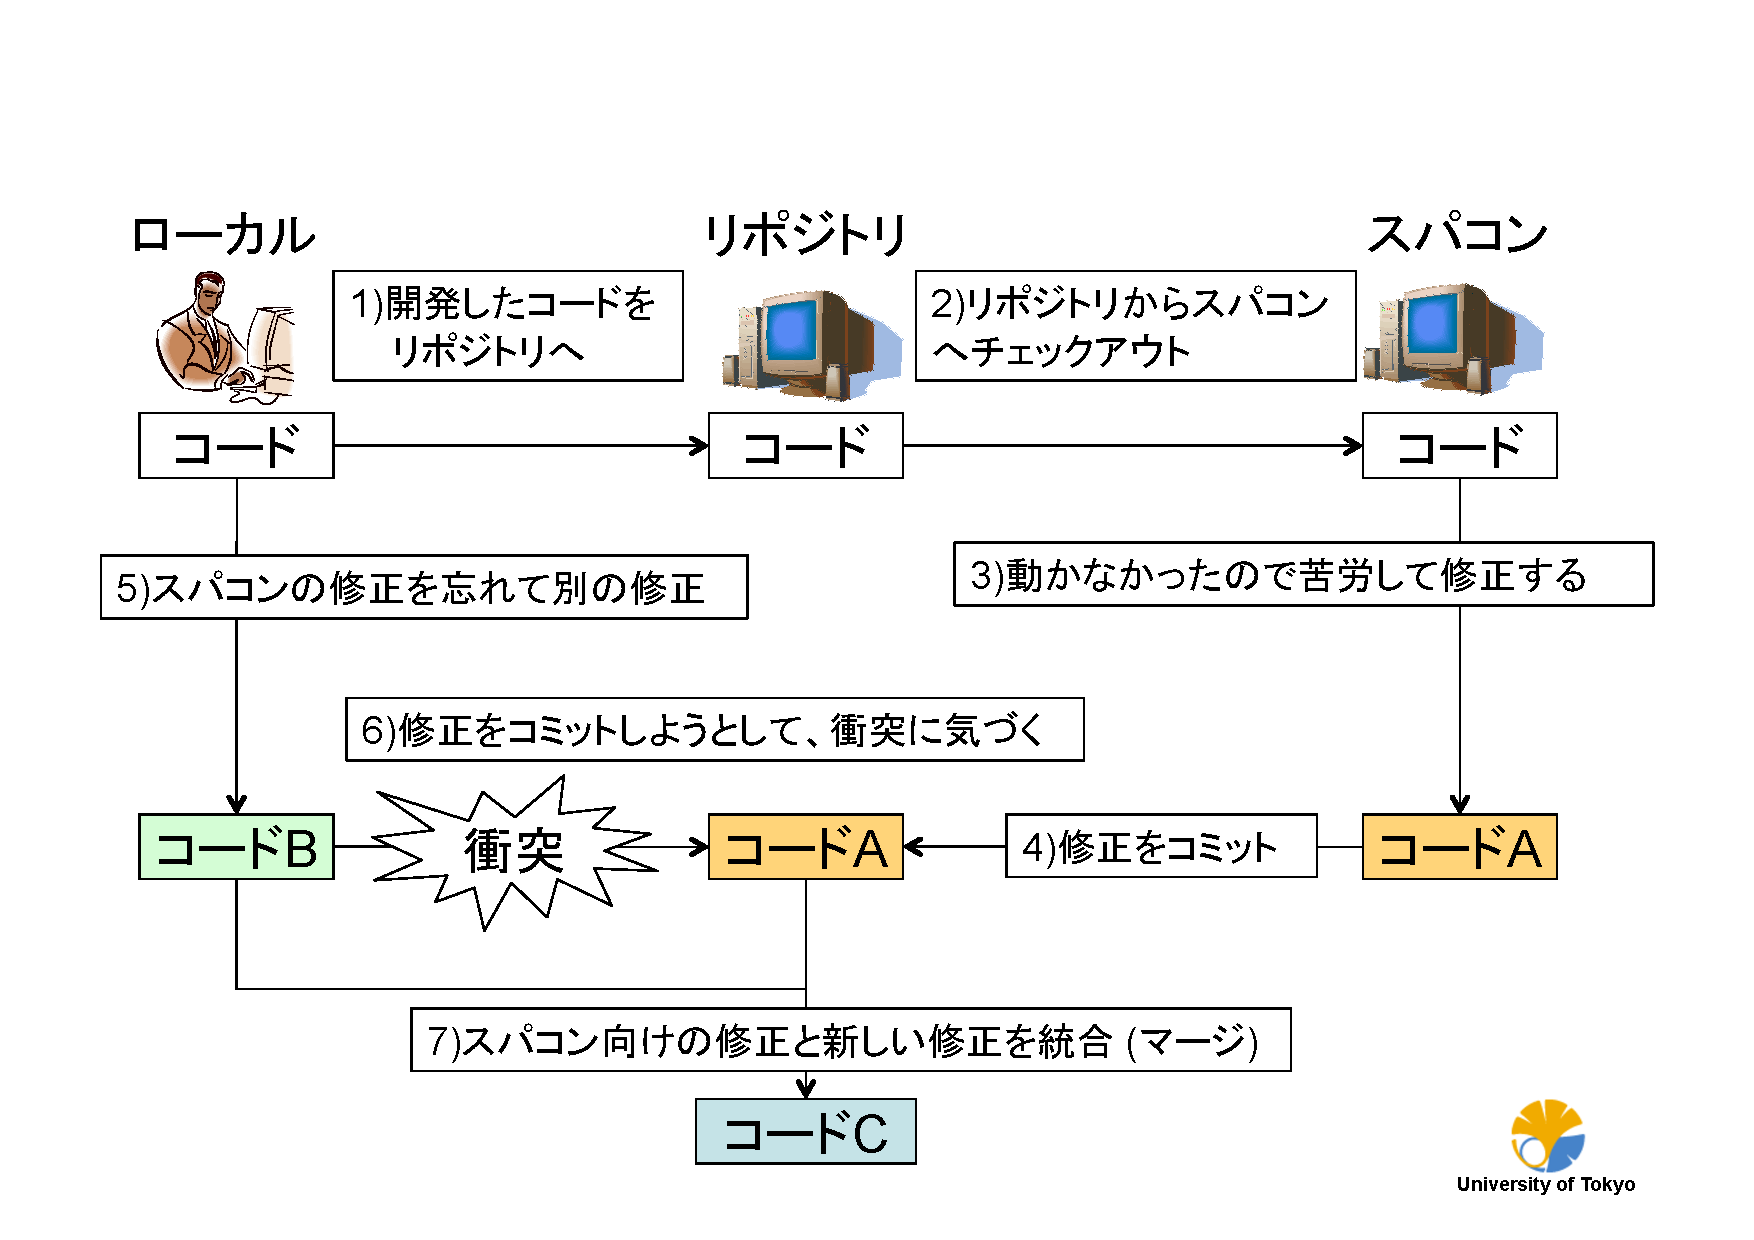
\includegraphics[height=0.88\textheight]{pattern-2.pdf}
  \end{center}
\end{frame}

\begin{frame}
  \frametitle{主なバージョン管理システム}
  \begin{itemize}
  \item BitKeeper - かつて Linux のカーネルのソース管理に使われていた
  \item CVS (Concurrent Versions System) - ネットワークでの利用を考慮とした初めてのバージョン管理システム。以前はよく使われていた
  \item Git - 現在 Linux の開発に使われている。分散型リポジトリ
  \item Mercurial - Git のライバル。分散型リポジトリ
  \item SCCS (Source Code Control System) - 70年代にベル研で開発された世界初のバージョン管理システム。現在は使われない
  \item Subversion - CVSの改良版として開発された。現在最もポピュラー? Mac OS X や多くの Linux には最初からインストールされている
  \end{itemize}
\end{frame}

\begin{frame}
  \frametitle{バージョン管理システムの欠点(面倒な点)}
  \begin{itemize}
  \item 修正前に最新の状態にアップデートしなければならない \\
   ⇒ 慣れると習慣になります
  \item 全ての修正を「コミット」しなければならない \\
    ⇒ 慣れると習慣になります
  \item 衝突(コンフリクト)が発生した時に対処しなければならない \\
    ⇒ 衝突に気づかずに修正してしまうほうが怖いです
  \item サーバのセットアップが面倒くさい \\
    ⇒ まずはホスティングサービス(sourceforge, github, bitbucket)を試してみましょう \\
    ⇒ まわりにいるプロ(?)に相談しましょう \\[.5em]
  \item バージョン管理システムを使うと作業効率が倍以上になる \\
    ⇒ {\color{red} 使わないと人生を半分損する}
  \end{itemize}
\end{frame}

\section{gitの基礎}

\begin{frame}
  \frametitle{gitの基礎}
  \begin{itemize}
  \item 「いつやるの? git入門」ページ28--34, 55, 58--110 \\
    \url{http://www.slideshare.net/matsukaz/git-17499005}
  \end{itemize}
\end{frame}

\begin{frame}
  \frametitle{実習: gitの基礎}
  \begin{itemize}
  \item ユーザ名などの設定
    git config user.name など
  \end{itemize}
\end{frame}

\section{ブランチとマージ}

\begin{frame}
  \frametitle{ブランチとマージ}
  \begin{itemize}
  \item 「いつやるの? git入門」ページ112--152 \\
    \url{http://www.slideshare.net/matsukaz/git-17499005}
  \item 「こわくないGit」ページ6--78 \\
    \url{http://www.slideshare.net/kotas/git-15276118}
  \end{itemize}
\end{frame}

\begin{frame}
  \frametitle{実習: ブランチとマージ}
\end{frame}

\section{リモートリポジトリとの連携}

\begin{frame}
  \frametitle{リモートリポジトリとの連携}
  \begin{itemize}
  \item 「いつやるの? git入門」ページ154--193 \\
    \url{http://www.slideshare.net/matsukaz/git-17499005}
  \end{itemize}
\end{frame}

\begin{frame}
  \frametitle{実習: リモートリポジトリとの連携}
  \begin{itemize}
  \item githubのリポジトリ
  \item (時間があれば)「Git道場 技 本日の課題、 テクニックの解説」 \\
    \url{https://speakerdeck.com/ogawa/git} に従って演習
  \end{itemize}
\end{frame}

\section{githubを用いたオープンソース・ソフトウェアの開発・公開}

\begin{frame}
  \frametitle{「公開ソフト」が備えているべきもの}
  \begin{itemize}
  \item マニュアル
  \item チュートリアル
  \item ライセンス
  \item ビルドシステム・インストーラー
    \begin{itemize}
    \item ソースコード配布 \\
      Linuxで一般的。ソースと一緒にビルド環境(Makefile, CMake, configure スクリプト)を配布
    \item バイナリ配布 \\
      Windowsで一般的。バイナリインストーラ形式で配布
    \end{itemize}
  \item ユーザフレンドリな操作環境(GUIなど)
  \item ユーザサポート体制
  \end{itemize}
\end{frame}

\begin{frame}
  \frametitle{ビルドシステム: CMake}
  \begin{itemize}
    \setlength{\itemsep}{1em}
  \item Makefileを生成するためのユーティリティー (configureスクリプトに対応)
    \begin{itemize}
    \item Windows の Visual C++ 用ソリューションファイル, Mac OS X の Xcode 用プロジェクトファイルの生成も可能
    \end{itemize}
  \item 設定は CMakeLists.txt に記述する
  \item テスト(CTest)やバイナリインストーラ作成(CPack)の機能もある
  \item ファイルの依存関係の自動検出
  \end{itemize}
\end{frame}

\end{document}
